\nomenclature{SoC}{System-on-Chip}
\nomenclature{OS}{Operating system}
\chapter{Requirements and specifications}\label{chapter:requirements}

This project goals include following the requirements stated by the Arcol company to the 360\degree vision system development. In this chapter both the software and hardware details are stated. The final system will be installed on the client bus using custom hardware. Thus, the designed software will have to adapt to the designed hardware constraints. Moreover, this Chapter also describes the requirements stated by the Arcol company to the final product.

\section{Hardware  and software specifications}
The final hardware consists on 4-6 cameras with the corresponding fisheye lenses, a board with a CPU and a FPGA, a TFT display and adapters set to interconnect the different devices to the board. The simplified hardware diagram is the following:

\begin{figure}[H]
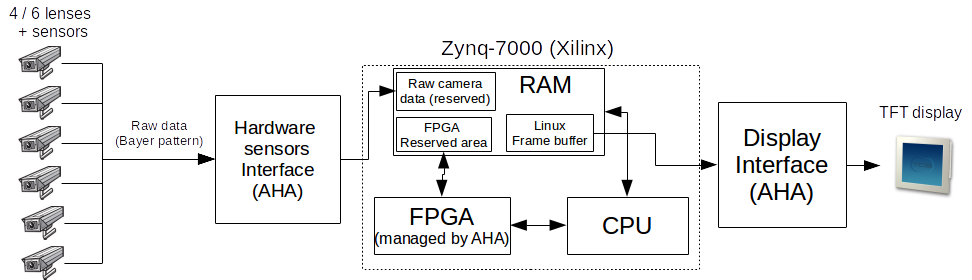
\includegraphics[scale=0.6]{images/hardwareDigram}
\caption{Arcol project hardware diagram}
\label{fig:hardwareDiag}
\end{figure}

The lenses used (Yuntai-optical  YT-5547-A1) have  178\degree (H) / 140\degree (V) viewing angle. The sensors (PixelPlus PH1100K) have an 1312$\times$816 effective resolution and provide the data in Bayer pattern. For each pixel only one color is provided, following the pattern shown in Figure~\ref{fig:bayer}. To obtain the full $M\times N$ image the color pixels are interpolated from its neighbours.

\begin{figure}
\center
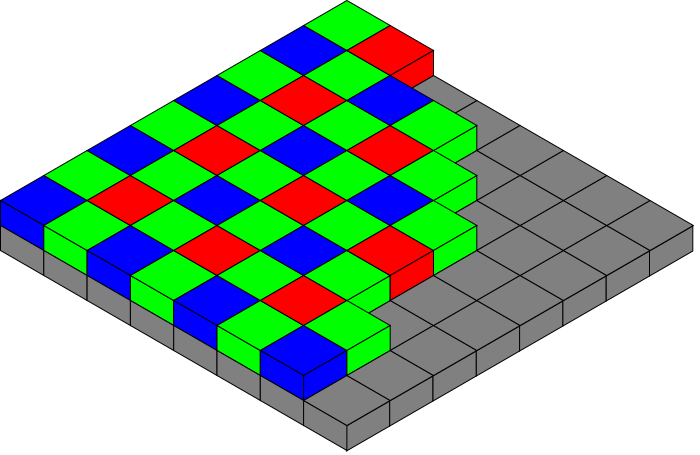
\includegraphics[scale=0.4]{images/bayer}
\caption{Camera sensor Bayer pattern. \cite{siliconimaging}}
\label{fig:bayer}
\end{figure}

This Bayer pattern data is stored in an specific RAM location by the driver and ready to be accessed by the software.  The evaluation board used in this project has an 8Mb RAM (Random Acces Memory). This memory is split between the OS (Operating system) kernel, the camera drivers and the FPGA. 

The board used (Xilinx Zynq-7000) has an ZC702 SoC (System-on-Chip) with two ARM cores and an FPGA,  1GB RAM DDR2 and a 16MB flash drive. Additionally, it has two FMC connectors used as camera input and display output with the AHA developed drivers.

Although this system can capture data from 6 cameras, only 4 cameras will be used in this TFG project. The remaining 2 cameras are reserved for future implementations --i.e. articulated buses.

All the developed software will not run directly on the Zynq board. Instead, an abstraction layer with a Linux kernel system will be installed. The software will run in the Linux user layer, and proper drivers to access the raw camera data and the FPGA reserved memory will be provided. 

The Linux OS will have OpenCV and Boost libraries installed. Thus, the software can use both libraries. Moreover, critical real-time and high parallelizable functions can be implemented on FPGA.

\section{Required features}\label{sec:algorithm}
Using the specified hardware/software combination stated before a stitching system will be developed. The resulting composite image must have the following properties:
\vspace{-1em}
\begin{description}[font=\normalfont\textsl]\itemsep2pt \parskip1pt \parsep0pt
\item [Non-discontinuities on ground lines --i.e. lane lanes.] The ground lines must neither be broken nor change its direction between cameras.
\item [Exposure compensation.] Perform a light correction between cameras.
\item [Avoid double-images or ghost images.] Objects located above ground --i.e. people--, cannot be occluded or seen double in the overlapped areas.
\end{description}
\vspace{-1em}
This project will focus on the warping process. Thus, only the first constraint will be taken into account.

Regarding the calibration step, there is a reasonably freedom to select the calibration pattern. However, this system has to be user friendly without decreasing the software performance. 